\documentclass[landscape]{article}
\usepackage{amsmath,amssymb,amsthm,graphicx,color}

\pagestyle{empty}

\headsep=0in
\parindent=0ex
\textwidth=8.5in
\textheight=6.0in

\oddsidemargin=0in


\newcommand{\slidetwo}[2]{\vfill
\eject
\centerline{\bf #1}
\bigskip
\centerline{\bf #2}
\vfill}

\newcommand{\slidethree}[3]{\vfill
\eject
\centerline{\bf #1}
\centerline{\bf #2}
\centerline{\bf #3}
\vfill}

\newcommand{\slide}[1]{
  \vfill
  \centerline{\Large\thepage}
  \eject
  \centerline{\bf #1}
  \vfill}

\newcommand{\slideplain}[1]{
  \vfill
  \centerline{\Large\thepage}
  \eject
  \centerline{\bf #1}
  \vfill}

\newcommand{\anaslide}[1]{
  \vfill
  \centerline{\Large\thepage}
  \eject \centerline{\bf #1}}

\newcommand{\anaslideplain}[1]{
  \vfill
  \eject
  \centerline{\bf #1}}

\newcommand{\bigsum}[2]{\mathop{{\huge \Sigma}}_{#1}^{#2}\;}

\newcommand{\tail}[1]{\Phi\left(#1\right)}

\newcommand{\Rmax}{R_{\max}}
\newcommand{\dmax}{d_{\max}}
\newcommand{\emax}{e_{\max}}
\newcommand{\domx}{{\cal X}}
\newcommand{\domy}{{\cal Y}}
\newcommand{\domr}{{\cal R}}

\newcommand{\var}[1]{\mbox{\tt{"}}#1\mbox{\tt{"}}}
\newcommand{\phrase}[1]{{\mathrm Phrase}(#1)}
\newcommand{\branch}[1]{{\mathrm Branch}(#1)}
\newcommand{\terminal}[1]{{\mathrm Terminal}(#1)}

\newcommand{\mtt}[1]{\mbox{\tt #1}}
\newtheorem{theorem}{\noindent Theorem}
\newtheorem{lemma}[theorem]{\noindent Lemma}
\newtheorem{observation}[theorem]{\noindent Observation}
\newtheorem{corollary}[theorem]{\noindent Corollary}
\newtheorem{conjecture}[theorem]{\noindent Conjecture}
\newtheorem{proposition}[theorem]{\noindent Proposition}
\newtheorem{example}{\noindent Example}
\newtheorem{definition}{\noindent Definition}
\newtheorem{claim}[theorem]{\noindent Claim}
\newtheorem{fact}[theorem]{\noindent Fact}

\DeclareMathOperator*{\argmax}{argmax}
\DeclareMathOperator*{\argmin}{argmin}
\DeclareMathOperator*{\softmax}{softmax}

\DeclareMathOperator*{\locmax}{locmax}
\DeclareMathOperator*{\locmin}{locmin}

\newcommand{\parens}[1]{\left(#1\right)}
\newcommand{\brackets}[1]{\left[#1\right]}
\newcommand{\nn}{\nonumber \\}

\newcommand{\expect}[1]{\mathrm{E}\left[#1\right]}
\newcommand{\expectsub}[2]{\mathrm{E}_{#1}\left[#2\right]}
\newcommand{\probsub}[2]{\mathrm{P}_{#1}\left[#2\right]}

\newcommand{\tuple}[1]{{\mbox{$\langle#1\rangle$}}}


\newcommand{\xmean}{\expect{X}}
\newcommand{\xxmean}{\overline{x}}
\newcommand{\sbound}{\tilde{\sigma}}
\newcommand{\betamin}{\beta_{\min}}
\newcommand{\betamax}{\beta_{\max}}
\newcommand{\xmin}{x_{\min}}
\newcommand{\xmax}{x_{\max}}
\newcommand{\expectbeta}[1]{\expectsub{\beta}{#1}}

\newcommand{\calx}{{\cal X}}
\newcommand{\caly}{{\cal Y}}

\newcommand{\dint}{\int\!\!\!\!\int}
\newcommand{\classcount}[1]{\mathrm{c}(#1)}
\newcommand{\smallprod}{{\prod}}

\newcommand{\ignore}[1]{}

\newcommand{\weight}[1]{{\mathrm Weight}(#1)}
\newcommand{\context}[1]{{\mathrm Context}(#1)}
\newcommand{\econtext}[1]{{\mathrm EContext}(#1)}
\newcommand{\sstop}{{\mathrm stop}}
\newcommand{\sstart}{{\mathrm start}}

\newcommand{\sidebyside}[2]{\parbox[t]{2.0in}{#1}\hspace{1.0in}
                            \parbox[t]{2.0in}{#2}}

\newcommand{\tightsidebyside}[2]{\parbox[t]{2.0in}{#1}\hspace{.3in}
                            \parbox[t]{2.0in}{#2}}

\newcommand{\subproves}[1]{\,\;\vdash\!\!_{#1}\;\,}

\def\irule#1#2#3#4{
\begin{tabbing}
#2 \parbox{.75in}{\noindent \hrule ~} $#3$ \\ #4
\end{tabbing}}

\def\ant#1{$#1$ \\}

\newcommand{\abs}{\text{\emph{abs}}}

\newcommand{\reals}{\mathbb{R}}

\newcommand{\pluseq}{\mbox{\tt +=}}

\newcommand{\minuseq}{\mbox{\tt -=}}

\newcommand{\grad}{\mathrm{grad}}
\begin{document}

{\Huge
  
  \centerline{\bf TTIC 31230, Fundamentals of Deep Learning}
  \bigskip
  \centerline{David McAllester, Winter 2018}
  \vfill
  \vfill
  \centerline{Multiclass Logistic Regression}
  \vfill
  \centerline{Multilayer Perceptrons}
  \vfill
  \centerline{Stochastic Gradient Descent (SGD)}
  \vfill
  \centerline{Computation Graphs and Backpropagation}
  \vfill
  \centerline{The Educational Framework (EDF)}
  \vfill
  \centerline{Minibatching}
  \vfill
  \vfill
  \vfill

\slide{Multiclass Classification}

We consider the problem of taking an input $x$ (such as an image of a hand written digit) and classifying it into some small number of classes (such as the digits $0$ through $9$).

\vfill
\centerline{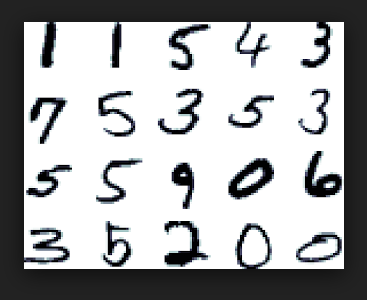
\includegraphics[width= 4.0in]{../images/MNIST}}
  
\slide{Multiclass Classification}

Assume a population distribution on pairs $(x,y)$ for $x \in \reals^d$ and $y \in {\cal C}$.

\vfill
For MNIST $x$ is a $28 \times 28$ image which we take to be a 784 dimensional vector giving $x \in \reals^{784}$.

\vfill
For MNIST ${\cal C}$ is the set $\{0,\ldots,9\}$.

\vfill
Assume a sample $(x_0,y_0),\;\ldots,\;(x_{N-1},y_{N-1})$ drawn IID from the population.

\vfill
We want to use the sample to construct a rule for predicting $y$ given $x$ when we draw new pairs from the population.

\slide{Multiclass Logistic Regression}

Assume a sample $(x_0,y_0),\;\ldots,\;(x_{N-1},y_{N-1})$ drawn IID from the population with $x \in \reals^d$ and $y \in \{0,\ldots,K\}$.

\vfill
For a new $x$ we compute a score $s(\hat{y})$ for each possible label $\hat{y}$.

\vfill
$$s = Wx + b$$

\slide{Multiclass Logistic Regression for MNIST}

$j$ --- image pixel

\vfill
$\hat{y}$ --- possible image label (0 through 9)

\vfill
$$s(\hat{y}) = \sum_j W[\hat{y},j]\; x[j] + b[\hat{y}]$$

\vfill
Note that $W[\hat{y},:]$ is an image.

\slide{Softmax}

Softmax converts scores (or energies or logits) to probabilities.

\vfill
\begin{eqnarray*}
  Q(\hat{y}) & = & \frac{1}{Z}\; e^{s(\hat{y})}
  \\
  \\
  \\
  Z & = & \sum_{\hat{y}} e^{s(\hat{y})}
\end{eqnarray*}

\vfill
In vector notation
\bigskip
$$Q  = \softmax\; s$$

\slide{Log Loss and Logistic Regression}
Let $Q_\Phi(\hat{y}|x)$ be defined by a model with parammeters $\Phi$.

\vfill
In logistic regression $\Phi$ is the pair $(W,b)$.

\vfill
Let $n$ range over training instances.

\begin{eqnarray*}
  W^*, b^* & = & \argmin_{W,b}\; \frac{1}{N} \sum_{n = 1}^N\;\;- \log Q_{W,b}(y_n|x_n) \\
  \\
  \\
  \Phi^* & = & \argmin_\Phi \;\frac{1}{N} \sum_{n = 1}^N\;\;- \log Q_\Phi(y_n|x_n) \\
\end{eqnarray*}


\slide{Information Theoretic Formulation}

Let $\Phi$ be the parameters of a probabilistc predictor $Q_\Phi$.

\vfill
\vfill
\centerline{We want \hspace{3ex} $\Phi^* = \argmin_\Phi \;\;\expectsub{(x,y) \sim {\cal P}}{ -\log Q_\Phi(y|x)}$.}

\vfill
\vfill
\vfill
This is {\bf cross-entropy} loss:

$$H({\cal P},{\cal Q}) = \expectsub{y \sim {\cal P}}{-\log\; {\cal Q}(y)}$$

$$H({\cal P}) = H({\cal P},{\cal P}) = \expectsub{y \sim {\cal P}}{-\log\; {\cal P}(y)}$$

$$H({\cal P},{\cal Q}) \geq H({\cal P})$$

$$\expectsub{(x,y) \sim {\cal P}}{ -\log Q_\Phi(y|x)} = \expectsub{x \sim {\cal P}}{H({\cal P}(:|x),Q_\Phi(:|x))}$$

\slide{Multi Layer Perceptrons (MLPs)}

Activation functions:
$$\sigma(u) = \frac{1}{1+e^{-u}}\;\;\;\;\;\;\;\;\mathrm{Relu}(u) = \max(u,0)$$

\vfill
\centerline{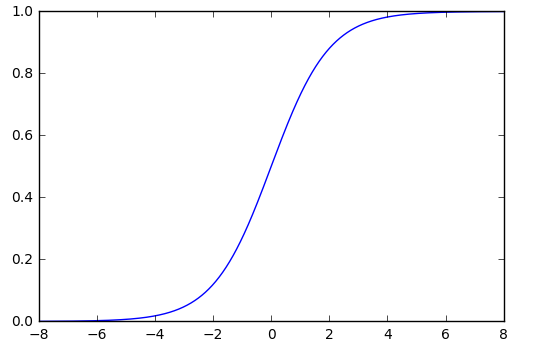
\includegraphics[width=1.5in]{../images/sigmoid}\hspace{1.0in}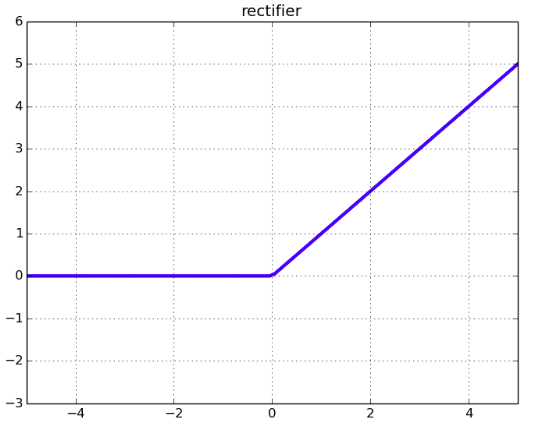
\includegraphics[width=1.2in]{../images/relu}}

\vfill
\begin{eqnarray*}
  L^0 & = & \mathrm{Relu}(W^0 x + b^0) \\
  \\
  L^1 & = & \sigma(W^1 L^0 + b^1) \\
  \\
  Q_\Phi & = & \softmax(L^1)
\end{eqnarray*}

\slide{Explicit Index Notation with {\em Typed Index Variables}}


$i$ --- pixels

$j$ --- image features

$\hat{y}$ --- possible image labels

\vfill
\begin{eqnarray*}
  L^0[j] & = & \mathrm{Relu}\left(\left(\sum_i\;W^0[j,i] \;x[i]\right) + b^0[j]\right) \\
  \\
  L^1[\hat{y}] & = & \sigma\left(\left(\sum_j\;W^1[\hat{y},j]\;L^0[j]\right) + b^1[\hat{y}]\right) \\
  \\
  Q_\Phi(\hat{y}) & = & \frac{1}{Z} \;e^{L^1[\hat{y}]}
\end{eqnarray*}

\ignore{
\slide{Index Types are Too Often Ignored}
For example: in Goodfellow et al. we have:


\centerline{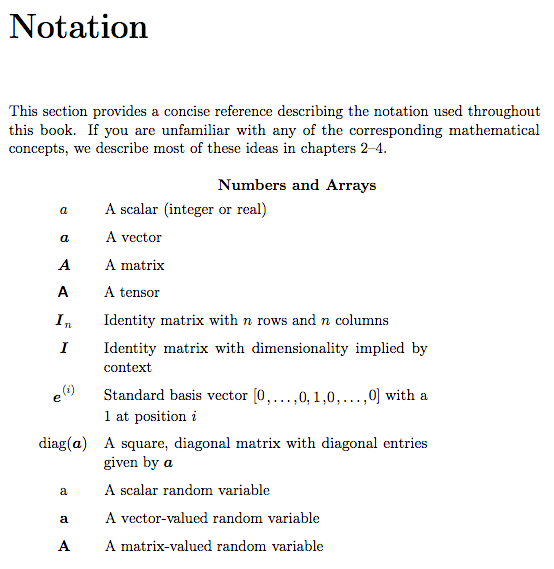
\includegraphics[height=5in]{../images/Notation}}

\slide{Abstract Optimization Problems}

Training minimizes (perhaps regularized) loss on the training data.

\vfill
$$\Phi^* = \argmin_\Phi\;\frac{1}{N} \sum_n \ell(\Phi,x_n,y_n)$$

\vfill
We would really like to minimize loss on the population.

\vfill
\vfill
$$\Phi^* = \argmin_\Phi\; E_{(x,y) \sim {\cal P}}\;\;\ell(\Phi,x,y)$$
}

\slide{Loss Vs. Error Rate}
While training (gradient descent) is generally done on log loss, performance is often judged by other measures such as error rate.

\vfill
The ``loss'' is often used as a synonym for log loss (or whatever loss defined the gradient descent training).

\vfill
Hence one often reports both ``loss'' and ``error rate''.

\vfill
Note that error rate is not differentiable.

\slide{Train Data, Development Data and Test Data}

Data is typically divided into {\bf a training set}, {\bf a development set} and {\bf a test set} each drawn IID from the population.

\vfill
A learning algorithm optimizes training loss.

\vfill
One then optimizes algorithm design (and hyper-parameters) on the development set. (graduate student descent).

\vfill
Ultimate performance should be done on a test set not used for development.  Test data is often withheld from developers.

\slide{Gradients with Respect to Systems of Parameters}

$\nabla_\Phi\;\ell(\Phi,x,y)$ denotes the partial derivative of $\ell(\Phi,x,y)$ with respect to the parameter system $\Phi$.

\vfill
Here can think of $\Phi$ as a single vector with
$$(\nabla_\Phi \;\ell(\Phi,x,y))_i = \partial \ell(\Phi,x,y) /\partial \Phi_i$$

\vfill
But in general $\Phi$ can be a multi-dimensional array (an ndarray in NumPy). If $\Phi$ is four dimensional we can write $\Phi[i,j,k,l]$.

\vfill
For scalar loss, $\nabla_\Phi \;\ell(\Phi,x,y)$ has the same shape as $\Phi$.

\vfill
$$\left(\nabla_\Phi \;\ell(\Phi,x,y)\right).\mathrm{shape} = \Phi.\mathrm{shape}$$

\slide{Total Gradient Descent}

$$\ell_{\mathrm{train}}(\Phi) = \frac{1}{N}\sum_n \ell(\Phi,x_n,y_n)$$

\vfill
\centerline{We want: \hspace{3ex} $\Phi^*  =  \argmin_\Phi \ell_{\mathrm{train}}(\Phi)$}

\vfill
$$\Phi \;\;\;\mbox{\tt -=}\;\;\; \eta \nabla_\Phi \ell_\mathrm{train}(\Phi)$$

\slide{Stochastic Gradient Descent (SGD) on the training set.}

\vfill
\vfill
repeat:  Select $n$ at random. $\Phi \;\;\minuseq\;\; \eta \;\nabla_\Phi \; \ell(\Phi,x_n,y_n)$

\begin{eqnarray*}
  \expectsub{n}{\nabla_\Phi \; \ell(\Phi,x_n,y_n)} & = & \sum_n P(n) \nabla_\Phi\;\ell_{\mathrm{train}}(\Phi,x_n,y_n) \\
  \\
  \\ & = & \frac{1}{N} \sum_n \nabla_\Phi\;\ell_{\mathrm{train}}(\Phi,x_n,y_n) \\
  \\
    \\ & = & \nabla_\Phi \frac{1}{N} \sum_n \;\ell_{\mathrm{train}}(\Phi,x_n,y_n) \\
  \\
  &  = & \nabla_\Phi\;\ell_{\mathrm{train}}(\Phi)
\end{eqnarray*}



\slide{Epochs}

In practice we cycle through the training data visiting each training pair once.

\vfill
One pass through the training data is called an Epoch.

\vfill
One typically imposes a random suffle of the training data before each epoch.

\slide{SGD for MLPs}

\centerline{$i$ --- image pixel \hspace{4ex} $j$ --- image feature \hspace{4ex} $\hat{y}$ --- possible label}

\vfill
\begin{eqnarray*}
  L^0[j] & = & \mathrm{Relu}\left(\left(\sum_i\;W^0[j,i] \;x[i]\right) + b^0[j]\right) \\
  \\
  L^1[\hat{y}] & = & \sigma\left(\left(\sum_j\;W^1[\hat{y},j]\;L^0[j]\right) + b^1[\hat{y}]\right) \\
  \\
  P(\hat{y}) & = & \frac{1}{Z} \;e^{L^1[\hat{y}]}
\end{eqnarray*}

\vfill
We now need $\frac{\partial \ell(\Phi,x,y)}{\partial \Phi[k]}$ for all $k$.

\slide{}

\centerline{Computation Graphs and Backpropagation}

\vfill

\slide{Computation Graphs}

A computation graph (sometimes called a ``computation{\color{red} al} graph'') is a sequence of assignment statements.


\vfill
\begin{eqnarray*}
  L^0[j] & = & \mathrm{Relu}\left(\left(\sum_i\;W^0[j,i] \;x[i]\right) + b^0[j]\right) \\
  \\
  L^1[\hat{y}] & = & \sigma\left(\left(\sum_j\;W^1[\hat{y},j]\;L^0[j]\right) + b^1[\hat{y}]\right) \\
  \\
  P(\hat{y}) & = & \frac{1}{Z} \;e^{L^1[\hat{y}]}
\end{eqnarray*}

\slide{Computation Graphs}
A simpler example:

\vfill
$$\ell = \sqrt{x^2 + y^2}$$
\begin{eqnarray*}
  u & = & x^2  \\
  v & = & y^2 \\
  r & =& u + v \\
  \ell & = & \sqrt{r}
\end{eqnarray*}

\vfill
A computation graph defines a DAG (a directed acyclic graph) where the variables are the nodes. Each assignment determines
one or more directed edges from the left hand variable to the right hand variables.

\anaslide{Computation Graphs}
\vspace{-1ex}
$$\begin{array}{lcl}
 1.\;u & = & x^2  \\
 2.\;w & = & y^2 \\
 3.\;r & =& u + w \\
  4.\;\ell & = & \sqrt{r}
\end{array}$$

\vfill
For each variable $z$ we can consider $\partial \ell/\partial z$.

\vfill
Gradients are computed in the reverse order.

\vfill
$$\begin{array}{lcl}
(4)\; \partial\ell/\partial r & = & \frac{1}{2\sqrt{r}} \\
(3)\; \partial\ell/\partial u & = & \partial \ell/\partial r \\
(3)\; \partial\ell/\partial w & = & \partial \ell/\partial r\\
(2)\; \partial\ell/\partial y & = & (\partial \ell/\partial w) * (2y) \\
(1)\; \partial\ell/\partial x & = & (\partial \ell/\partial u) * (2x)
\end{array}$$

\anaslide{A More Abstract Example}
\vspace{-3ex}
\begin{eqnarray*}
  y & = & f(x) \\
  z & = & g(y,x) \\
  u & = & h(z) \\
  \ell & = & u
\end{eqnarray*}

\medskip
For now assume all values are scalars.

\medskip
We will ``backpopagate'' the assignments the reverse order.

\anaslide{Backpropagation}
\vspace{-3ex}
\begin{eqnarray*}
  y & = & f(x) \\
  z & = & g(y,x) \\
  u & = & h(z) \\
  \ell &  = & {\color{red} u}
\end{eqnarray*}

\medskip
{\color{red} ${\partial \ell}/{\partial u} = 1$}

\anaslide{Backpropagation}
\vspace{-3ex}
\begin{eqnarray*}
  y & = & f(x) \\
  z & = & g(y,x) \\
  u & = & h({\color{red} z}) \\
  \ell &  = &  u
\end{eqnarray*}

\medskip
${\partial \ell}/{\partial u} = 1$

\medskip
{\color{red} ${\partial \ell}/{\partial z} = ({\partial \ell}/{\partial u})\; ({\partial h}/{\partial z})$} (this uses the value of $z$)

\anaslide{Backpropagation}
\vspace{-3ex}
\begin{eqnarray*}
  y & = & f(x) \\
  z & = & g({\color{red} y},x) \\
  u & = & h(z) \\
  \ell &  = &  u
\end{eqnarray*}

\medskip
${\partial \ell}/{\partial u} = 1$

\medskip
${\partial \ell}/{\partial z} = ({\partial \ell}/{\partial u})\; ({\partial h}/{\partial z})$

\medskip
{\color{red} ${\partial \ell}/{\partial y} = ({\partial \ell}/{\partial z})\; ({\partial g}/{\partial y})$} (this uses the value of $y$ and $x$)

\anaslide{Backpropagation}
\vspace{-3ex}
\begin{eqnarray*}
  y & = & f({\color{red} x}) \\
  z & = & g(y,{\color{red} x}) \\
  u & = & h(z) \\
  \ell &  = &  u
\end{eqnarray*}

\medskip
${\partial \ell}/{\partial u} = 1$

\medskip
${\partial \ell}/{\partial z} = ({\partial \ell}/{\partial u})\; ({\partial h}/{\partial z})$

\medskip
${\partial \ell}/{\partial y} = ({\partial \ell}/{\partial z})\; ({\partial g}/{\partial y})$

\medskip
{\color{red} ${\partial \ell}/{\partial x} =$ ???} Oops, we need to add up multiple occurrences.

\anaslide{Backpropagation}
\vspace{-3ex}
\begin{eqnarray*}
  y & = & f({\color{red} x}) \\
  z & = & g(y,{\color{red} x}) \\
  u & = & h(z) \\
  \ell &  = &  u
\end{eqnarray*}

\medskip
We let {\color{red} $x.\grad$} be an attribute (as in Python) of node {\color{red} $x$}.

\bigskip
\bigskip
We will initialize {\color{red} $x.\mathrm{grad}$} to zero.

\bigskip
\bigskip
During backpropagation we will accumulate contributions to {\color{red} ${\partial \ell}/{\partial x}$} into {\color{red} $x.\grad$}.


\anaslide{Backpropagation}
\vspace{-3ex}
\begin{eqnarray*}
  y & = & f(x) \\
  z & = & g(y,x) \\
  u & = & h(z) \\
  {\color{red} \ell} &  {\color{red} =} & {\color{red}  u}
\end{eqnarray*}


\medskip
$z.\grad = y.\grad = x.\grad = 0$

\medskip
$u.\grad = 1$

\medskip
{\bf Loop Invariant}: For any variable $w$ whose definition has not yet been processed we have that $w.\grad$ is $\partial \ell/\partial w$ as defined by the set of assignments already processed.

\anaslide{Backpropagation}
\vspace{-3ex}
\begin{eqnarray*}
  y & = & f(x) \\
  z & = & g(y,x) \\
  {\color{red} u} & {\color{red} =} & {\color{red} h(z)} \\
  {\color{red} \ell} & {\color{red}  =} &  {\color{red} u}
\end{eqnarray*}

\medskip
$z.\grad = y.\grad = x.\grad = 0$

\medskip
$u.\grad = 1$

\medskip
{\bf Loop Invariant}: For any variable $w$ whose definition has not yet been processed we have that $w.\grad$ is $\partial \ell/\partial w$ as defined by the set of assignments already processed.

\medskip
$z.\grad\;\pluseq\; u.\grad * {\partial h}/{\partial z}$

\anaslide{Backpropagation}
\vspace{-3ex}
\begin{eqnarray*}
  y & = & f(x) \\
  {\color{red} z} & {\color{red} =} & {\color{red} g(y,x)} \\
  {\color{red} u} & {\color{red} =} & {\color{red} h(z)} \\
  {\color{red} \ell} & {\color{red} =} & {\color{red}  u}
\end{eqnarray*}

\medskip
$z.\grad = y.\grad = x.\grad = 0$

\medskip
$u.\grad = 1$

\medskip
    {\bf Loop Invariant}: For any variable $w$ whose definition has not yet been processed we have that $w.\grad$ is $\partial \ell/\partial w$ as defined by the set of assignments already processed.

\medskip
$z.\grad\;\pluseq\; u.\grad * {\partial h}/{\partial z}$

\medskip
$y.\grad \;\pluseq\; z.\grad * {\partial g}/{\partial y}$

\medskip
$x.\grad \;\pluseq\; z.\grad * {\partial g}/{\partial x}$

\anaslideplain{Backpropagation}
\vspace{-3ex}
\begin{eqnarray*}
  {\color{red} y} & {\color{red} =} & {\color{red} f(x)} \\
  {\color{red} z} & {\color{red} =} & {\color{red} g(y,x)} \\
  {\color{red} u} & {\color{red} =} & {\color{red} h(z)} \\
  {\color{red} \ell} & {\color{red} =} & {\color{red} u}
\end{eqnarray*}

\medskip
$z.\grad = y.\grad = x.\grad = 0$

\medskip
$u.\grad = 1$

\medskip
$z.\grad\;\pluseq\; u.\grad * {\partial h}/{\partial z}$

\medskip
$y.\grad \;\pluseq\; z.\grad * {\partial g}/{\partial y}$

\medskip
$x.\grad \;\pluseq\; z.\grad * {\partial g}/{\partial x}$

\medskip
$x.\grad \;\pluseq\; y.\grad * {\partial f}/{\partial x}$

\anaslide{The Vector-Valued Case}
\vspace{-3ex}
\begin{eqnarray*}
  y & = & f(x) \\
  z & = & g(y,x) \\
  u & = & h(z) \\
  \ell & = & u
\end{eqnarray*}

\vfill
Now suppose the variables can be  vector-valued.

\vfill
The loss $\ell$ is still a scalar.

\vfill
In this case
$$x.\mathrm{grad} = \nabla_x\;\ell$$

\vfill
These are now vectors of the same dimension with
$$x.\mathrm{grad}[i] = \partial \ell/\partial x[i]$$

\slide{The Jacobian Matrix}
Consider $y =f(x)$ in vector-valued case.
\vfill
In the vector-valued case the backpropagation equation is
\vfill
$$x.\mathrm{grad}\; \mbox{\tt +=}\; (y.\mathrm{grad})^\top\; \nabla_x f(x)$$
\vfill
where
$$(\nabla_x f(x))[i,j] = {\cal J}[i,j] = \partial f(x)[i] /\partial x[j]$$

\vfill
The matrix ${\cal J}[i,j]$ is the Jacobian of $f$.

\vfill
Index Types: $j$ is an $x$-index and $i$ is a $y$-index.

\slide{The Tensor-Valued Case}

\begin{eqnarray*}
  y & = & f(x) \\
  z & = & g(y,x) \\
  u & = & h(z) \\
  \ell & = & u
\end{eqnarray*}

\vfill
Now suppose the variables can be  tensor-valued (the values are multi-dimensional arrays).  The loss is still a scalar.

\vfill
The computation is now a ``tensor flow''.

\slide{The Tensor-Valued Case}
For the tensor case we simply view tensors as a special case of vectors.  The indeces of $x.\mathrm{grad}$ are the
same as the indeces of $x$.
$$x.\mathrm{grad}.\mathrm{shape} = x.\mathrm{shape}$$

\vfill
The backpropagation equation for $y = f(x)$ is

$$x.\mathrm{grad}[i_1,\ldots,i_n] = (y.\mathrm{grad})[j_1,\ldots,j_k] \nabla_x f(x)[j_1,\ldots,j_k,i_1,\ldots,i_n]$$

\vfill
$j_1,\ldots,j_k$ are indeces of $y$ and $i_1,\ldots,i_n$ are indeces of $x$.

\vfill
Indeces not on the left of the equation are implicitly summed.

\anaslide{The EDF Framework}

The educational frameword (EDF) is a simple Python-NumPy implementation of a ``framework'' for defining computation graphs
and performing backpropagation. In EDF we write
\begin{eqnarray*}
  y & = & F(x) \\
  z & = & G(y,x) \\
  u & = & H(z) \\
  \ell &  = &  u
\end{eqnarray*}
\medskip
This is Python code where variables are bound to objects.

\anaslide{The EDF Framework}

The educational frameword (EDF) is a simple Python-NumPy implementation of a ``framework'' for defining computation graphs
and performing backpropagation. In EDF we write
\begin{eqnarray*}
  y & = & F(x) \\
  z & = & G(y,x) \\
  u & = & H(z) \\
  \ell &  = &  u
\end{eqnarray*}
\medskip
This is Python code where variables are bound to objects.

\medskip
$x$ is an object in the class {\tt Input}.

\medskip
$y$ is an object in the class $F$.

\medskip
$z$ is an object in the class $G$.

\medskip
$u$ and $\ell$ are the same object in the class $H$.

\anaslideplain{$y = F(x)$}

\begin{tabbing}
  class \=$F$(CompNode): \\
  \\
    \>def \=\_\_init\_\_(self, x): \\
        \>\>CompNodes.append(self) \\
        \>\>self.x = x \\
\\
    \>def forward(self): \\
        \>\>self.value = f(self.x.value) \\
\\
    \>def backward(self): \\
        \>\>self.x.addgrad(self.grad$ \;*\; \nabla_x\;f(x)$) \hspace{2em} \#needs x.value
\end{tabbing}

\slide{Nodes of the Computation Graph}

There are three kinds of nodes in a computation graph --- inputs, parameters and computation nodes.

\vfill
\begin{tabbing}
class \=Input: \\
    \>def \=\_\_init\_\_(self): \\
        \>\>pass \\
    \>def \>addgrad(self, delta): \\
    \>\>pass
\end{tabbing}

\vfill
\begin{tabbing}
class \=CompNode: \#initialization is handled by the subclass \\
   \>def \=addgrad(self, delta): \\
   \>\>self.grad += delta
\end{tabbing}

\slide{}

\begin{tabbing}
class \=Parameter: \\
    \\
    \>def \=\_\_init\_\_(self,value): \\
        \>\>Parameters.append(self) \\
        \>\>self.value = value \\
\\
    \>def \>addgrad(self, delta): \\
          \>\>\#sums over the minibatch \\
    \>\>self.grad += np.sum(delta, axis = 0) \\
    \\
    \>def \>SGD(self): \\
    \>\>self.value -= learning\_rate*self.grad
\end{tabbing}

\anaslide{MLP in EDF}
\medskip

The following Python code constructs the computation graph of a multi-layer perceptron (NLP) with one hidden layer.

\vfill
\begin{verbatim}
  L1 = Relu(Affine(Phi1,x))
  Q = Softmax(Sigmoid(Affine(Phi2,L1))
  ell = LogLoss(Q,y)
\end{verbatim}

\vfill
Here {\tt x} and {\tt y} are input computation nodes
whose value have been set.
Here {\tt Phi1} and {\tt Phi2} are ``parameter packages'' (a matrix and a bias vector in this case).
We have computation node classes {\tt Affine}, {\tt Relu}, {\tt Sigmoid}, {\tt LogLoss} each of which has
a forward and a backward method.

\vfill
\eject
\begin{verbatim}
class Affine(CompNode):

    def __init__(self,Phi,x):
        CompNodes.append(self)
        self.x = x
        self.Phi = Phi

    def forward(self):
        self.value = (np.matmul(self.x.value,
                               self.Phi.w.value)
                      + self.Phi.b.value)
\end{verbatim}
\vfill
\eject
\vfill
\begin{verbatim}
    def backward(self):

        self.x.addgrad(
           np.matmul(self.grad,
                     self.Phi.w.value.transpose()))

        self.Phi.b.addgrad(self.grad)

        self.Phi.w.addgrad(self.x.value[:,:,np.newaxis]
                           * self.grad[:,np.newaxis,:])
\end{verbatim}

\slide{The Core of EDF}

\begin{verbatim}
def Forward():
    for c in CompNodes: c.forward()

def Backward(loss):
    for c in CompNodes + Parameters: c.grad = 0
    loss.grad = 1/nBatch
    for c in CompNodes[::-1]: c.backward()

def SGD():
    for p in Parameters:
        p.SGD()
\end{verbatim}
\vfill

\slide{Minibatching}

Ther running time of EDF, and of any framework, is greatly improved by minibatching.

 \vfill
{\bf Minibatching}: We run some number of instances together (or in parallel) and then do a parameter update based on the average
gradients of the instances of the batch.

\vfill
For NumPy minibatching is not so much about parallelism as about making the vector operations larger so that the vector operations dominate
the slowness of Python.  On a GPU minibatching allows parallelism over the batch elements.
\vfill

\slide{Minibatching}
\vfill
With minibatching each input value and each computed value is actually a batch of values.

\vfill
We add a batch index as an additional first tensor dimensionfor each input and computed node.

\vfill
For example, if a given input is a $D$-dimensional vector then the value of an input node
has shape $(B,D)$ where $B$ is size of the minibatch.

\vfill
Parameters do not have a batch index.

\vfill
\eject
\vfill
\begin{tabbing}
class \=Parameter: \\
    \\
    \>def \=\_\_init\_\_(self,value): \\
        \>\>Parameters.append(self) \\
        \>\>self.value = value \\
\\
    \>def \>addgrad(self, delta): \\
          \>\>\#sums over the minibatch \\
    \>\>self.grad += np.sum(delta, axis = 0) \\
    \\
    \>def \>SGD(self): \\
    \>\>self.value -= learning\_rate*self.grad
\end{tabbing}

\slide{forward and backward must handle minibatching}

The forward and backward methods must be written to handle minibatching.  We will consider some examples.


\slide{An MLP}

\vfill
\begin{verbatim}
  L1 = Relu(Affine(Phi1,x))
  P = Softmax(Sigmoid(Affine(Phi2,L1))
  ell = LogLoss(P,y)
\end{verbatim}


\slide{The {\tt Sigmoid} Class}

The Sigmoid and Relu classes just work.

\begin{verbatim}
class Sigmoid:
    def __init__(self,x):
        CompNodes.append(self)
        self.x = x

    def forward(self):
        self.value = 1. / (1. + np.exp(-self.x.value))

    def backward(self):
        self.x.grad += self.grad
                       * self.value
                       * (1.-self.value)
\end{verbatim}


\vfill
\eject
\begin{verbatim}
y = Affine([W,B],x)

 forward:
  y.value[b,j] = x.value[b,i]W.value[i,j]
  y.value[b,j] += B.value[j]

 backward:
    x.grad[b,i] += y.grad[b,j]W.value[i,j]
    W.grad[i,j] += y.grad[b,j]x.value[i]
    B.grad[j] += y.grad[b,j]
\end{verbatim}

\vfill
\eject
\begin{verbatim}
class Affine(CompNode):

    def __init__(self,Phi,x):
        CompNodes.append(self)
        self.x = x
        self.Phi = Phi

    def forward(self):
        # y.value[b,j] = x.value[b,i]W.value[i,j]
        # y.value[b,j] += B.value[j]
        self.value = (np.matmul(self.x.value,
                                self.Phi.W.value)
                      + self.Phi.B.value)
\end{verbatim}
\vfill
\eject
\vfill
\begin{verbatim}
    def backward(self):

        self.x.addgrad(
           # x.grad[b,i] += y.grad[b,j]W.value[i,j]
           np.matmul(self.grad,
                     self.Phi.W.value.transpose()))

        # B.grad[j] += y.grad[b,j]
        self.Phi.B.addgrad(self.grad)

        # W.grad[i,j] += y.grad[b,j]x.value[b,i]
        self.Phi.W.addgrad(self.x.value[:,:,np.newaxis]
                           * self.grad[:,np.newaxis,:])
\end{verbatim}

\slide{END}
}
\end{document}
